\documentclass[1p]{elsarticle_modified}
%\bibliographystyle{elsarticle-num}

%\usepackage[colorlinks]{hyperref}
%\usepackage{abbrmath_seonhwa} %\Abb, \Ascr, \Acal ,\Abf, \Afrak
\usepackage{amsfonts}
\usepackage{amssymb}
\usepackage{amsmath}
\usepackage{amsthm}
\usepackage{scalefnt}
\usepackage{amsbsy}
\usepackage{kotex}
\usepackage{caption}
\usepackage{subfig}
\usepackage{color}
\usepackage{graphicx}
\usepackage{xcolor} %% white, black, red, green, blue, cyan, magenta, yellow
\usepackage{float}
\usepackage{setspace}
\usepackage{hyperref}

\usepackage{tikz}
\usetikzlibrary{arrows}

\usepackage{multirow}
\usepackage{array} % fixed length table
\usepackage{hhline}

%%%%%%%%%%%%%%%%%%%%%
\makeatletter
\renewcommand*\env@matrix[1][\arraystretch]{%
	\edef\arraystretch{#1}%
	\hskip -\arraycolsep
	\let\@ifnextchar\new@ifnextchar
	\array{*\c@MaxMatrixCols c}}
\makeatother %https://tex.stackexchange.com/questions/14071/how-can-i-increase-the-line-spacing-in-a-matrix
%%%%%%%%%%%%%%%

\usepackage[normalem]{ulem}

\newcommand{\msout}[1]{\ifmmode\text{\sout{\ensuremath{#1}}}\else\sout{#1}\fi}
%SOURCE: \msout is \stkout macro in https://tex.stackexchange.com/questions/20609/strikeout-in-math-mode

\newcommand{\cancel}[1]{
	\ifmmode
	{\color{red}\msout{#1}}
	\else
	{\color{red}\sout{#1}}
	\fi
}

\newcommand{\add}[1]{
	{\color{blue}\uwave{#1}}
}

\newcommand{\replace}[2]{
	\ifmmode
	{\color{red}\msout{#1}}{\color{blue}\uwave{#2}}
	\else
	{\color{red}\sout{#1}}{\color{blue}\uwave{#2}}
	\fi
}

\newcommand{\Sol}{\mathcal{S}} %segment
\newcommand{\D}{D} %diagram
\newcommand{\A}{\mathcal{A}} %arc


%%%%%%%%%%%%%%%%%%%%%%%%%%%%%5 test

\def\sl{\operatorname{\textup{SL}}(2,\Cbb)}
\def\psl{\operatorname{\textup{PSL}}(2,\Cbb)}
\def\quan{\mkern 1mu \triangleright \mkern 1mu}

\theoremstyle{definition}
\newtheorem{thm}{Theorem}[section]
\newtheorem{prop}[thm]{Proposition}
\newtheorem{lem}[thm]{Lemma}
\newtheorem{ques}[thm]{Question}
\newtheorem{cor}[thm]{Corollary}
\newtheorem{defn}[thm]{Definition}
\newtheorem{exam}[thm]{Example}
\newtheorem{rmk}[thm]{Remark}
\newtheorem{alg}[thm]{Algorithm}

\newcommand{\I}{\sqrt{-1}}
\begin{document}

%\begin{frontmatter}
%
%\title{Boundary parabolic representations of knots up to 8 crossings}
%
%%% Group authors per affiliation:
%\author{Yunhi Cho} 
%\address{Department of Mathematics, University of Seoul, Seoul, Korea}
%\ead{yhcho@uos.ac.kr}
%
%
%\author{Seonhwa Kim} %\fnref{s_kim}}
%\address{Center for Geometry and Physics, Institute for Basic Science, Pohang, 37673, Korea}
%\ead{ryeona17@ibs.re.kr}
%
%\author{Hyuk Kim}
%\address{Department of Mathematical Sciences, Seoul National University, Seoul 08826, Korea}
%\ead{hyukkim@snu.ac.kr}
%
%\author{Seokbeom Yoon}
%\address{Department of Mathematical Sciences, Seoul National University, Seoul, 08826,  Korea}
%\ead{sbyoon15@snu.ac.kr}
%
%\begin{abstract}
%We find all boundary parabolic representation of knots up to 8 crossings.
%
%\end{abstract}
%\begin{keyword}
%    \MSC[2010] 57M25 
%\end{keyword}
%
%\end{frontmatter}

%\linenumbers
%\tableofcontents
%
\newcommand\colored[1]{\textcolor{white}{\rule[-0.35ex]{0.8em}{1.4ex}}\kern-0.8em\color{red} #1}%
%\newcommand\colored[1]{\textcolor{white}{ #1}\kern-2.17ex	\textcolor{white}{ #1}\kern-1.81ex	\textcolor{white}{ #1}\kern-2.15ex\color{red}#1	}

{\Large $\underline{12n_{0157}~(K12n_{0157})}$}

\setlength{\tabcolsep}{10pt}
\renewcommand{\arraystretch}{1.6}
\vspace{1cm}\begin{tabular}{m{100pt}>{\centering\arraybackslash}m{274pt}}
\multirow{5}{120pt}{
	\centering
	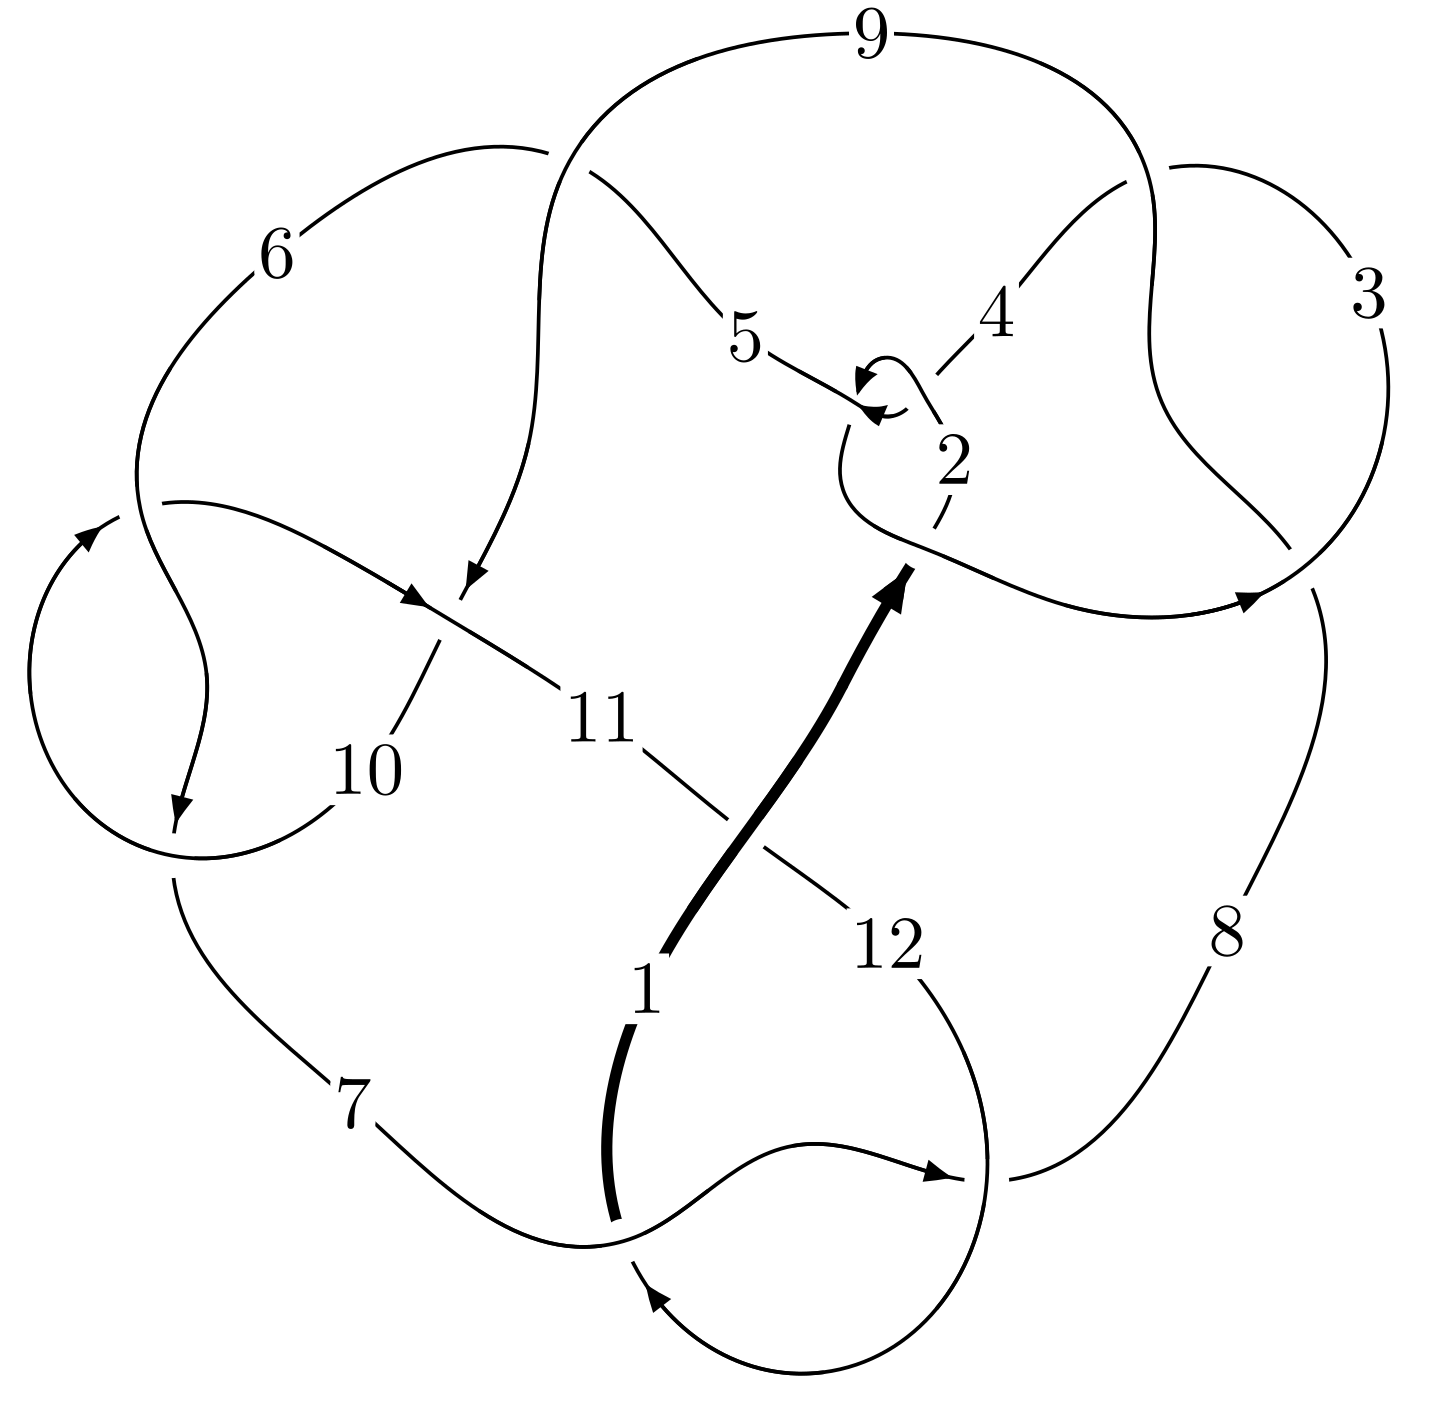
\includegraphics[width=112pt]{../../../GIT/diagram.site/Diagrams/png/2246_12n_0157.png}\\
\ \ \ A knot diagram\footnotemark}&
\allowdisplaybreaks
\textbf{Linearized knot diagam} \\
\cline{2-2}
 &
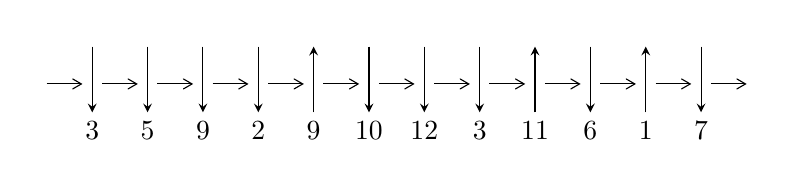
\begin{tikzpicture}[x=20pt, y=17pt]
	% nodes
	\node (C0) at (0, 0) {};
	\node (C1) at (1, 0) {};
	\node (C1U) at (1, +1) {};
	\node (C1D) at (1, -1) {3};

	\node (C2) at (2, 0) {};
	\node (C2U) at (2, +1) {};
	\node (C2D) at (2, -1) {5};

	\node (C3) at (3, 0) {};
	\node (C3U) at (3, +1) {};
	\node (C3D) at (3, -1) {9};

	\node (C4) at (4, 0) {};
	\node (C4U) at (4, +1) {};
	\node (C4D) at (4, -1) {2};

	\node (C5) at (5, 0) {};
	\node (C5U) at (5, +1) {};
	\node (C5D) at (5, -1) {9};

	\node (C6) at (6, 0) {};
	\node (C6U) at (6, +1) {};
	\node (C6D) at (6, -1) {10};

	\node (C7) at (7, 0) {};
	\node (C7U) at (7, +1) {};
	\node (C7D) at (7, -1) {12};

	\node (C8) at (8, 0) {};
	\node (C8U) at (8, +1) {};
	\node (C8D) at (8, -1) {3};

	\node (C9) at (9, 0) {};
	\node (C9U) at (9, +1) {};
	\node (C9D) at (9, -1) {11};

	\node (C10) at (10, 0) {};
	\node (C10U) at (10, +1) {};
	\node (C10D) at (10, -1) {6};

	\node (C11) at (11, 0) {};
	\node (C11U) at (11, +1) {};
	\node (C11D) at (11, -1) {1};

	\node (C12) at (12, 0) {};
	\node (C12U) at (12, +1) {};
	\node (C12D) at (12, -1) {7};
	\node (C13) at (13, 0) {};

	% arrows
	\draw[->,>={angle 60}]
	(C0) edge (C1) (C1) edge (C2) (C2) edge (C3) (C3) edge (C4) (C4) edge (C5) (C5) edge (C6) (C6) edge (C7) (C7) edge (C8) (C8) edge (C9) (C9) edge (C10) (C10) edge (C11) (C11) edge (C12) (C12) edge (C13) ;	\draw[->,>=stealth]
	(C1U) edge (C1D) (C2U) edge (C2D) (C3U) edge (C3D) (C4U) edge (C4D) (C5D) edge (C5U) (C6U) edge (C6D) (C7U) edge (C7D) (C8U) edge (C8D) (C9D) edge (C9U) (C10U) edge (C10D) (C11D) edge (C11U) (C12U) edge (C12D) ;
	\end{tikzpicture} \\
\hhline{~~} \\& 
\textbf{Solving Sequence} \\ \cline{2-2} 
 &
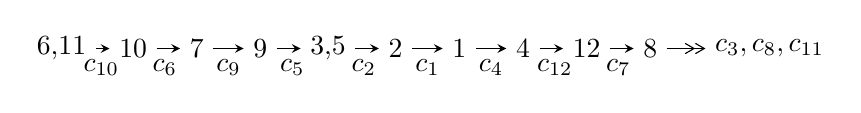
\begin{tikzpicture}[x=23pt, y=7pt]
	% node
	\node (A0) at (-1/8, 0) {6,11};
	\node (A1) at (1, 0) {10};
	\node (A2) at (2, 0) {7};
	\node (A3) at (3, 0) {9};
	\node (A4) at (65/16, 0) {3,5};
	\node (A5) at (41/8, 0) {2};
	\node (A6) at (49/8, 0) {1};
	\node (A7) at (57/8, 0) {4};
	\node (A8) at (65/8, 0) {12};
	\node (A9) at (73/8, 0) {8};
	\node (C1) at (1/2, -1) {$c_{10}$};
	\node (C2) at (3/2, -1) {$c_{6}$};
	\node (C3) at (5/2, -1) {$c_{9}$};
	\node (C4) at (7/2, -1) {$c_{5}$};
	\node (C5) at (37/8, -1) {$c_{2}$};
	\node (C6) at (45/8, -1) {$c_{1}$};
	\node (C7) at (53/8, -1) {$c_{4}$};
	\node (C8) at (61/8, -1) {$c_{12}$};
	\node (C9) at (69/8, -1) {$c_{7}$};
	\node (A10) at (11, 0) {$c_{3},c_{8},c_{11}$};

	% edge
	\draw[->,>=stealth]	
	(A0) edge (A1) (A1) edge (A2) (A2) edge (A3) (A3) edge (A4) (A4) edge (A5) (A5) edge (A6) (A6) edge (A7) (A7) edge (A8) (A8) edge (A9) ;
	\draw[->>,>={angle 60}]	
	(A9) edge (A10);
\end{tikzpicture} \\ 

\end{tabular} \\

\footnotetext{
The image of knot diagram is generated by the software ``\textbf{Draw programme}" developed by Andrew Bartholomew(\url{http://www.layer8.co.uk/maths/draw/index.htm\#Running-draw}), where we modified some parts for our purpose(\url{https://github.com/CATsTAILs/LinksPainter}).
}\phantom \\ \newline 
\centering \textbf{Ideals for irreducible components\footnotemark of $X_{\text{par}}$} 
 
\begin{align*}
I^u_{1}&=\langle 
u^{16}-3 u^{15}+6 u^{14}-8 u^{13}+12 u^{12}-12 u^{11}+12 u^{10}-3 u^9-3 u^8+5 u^7-9 u^6+9 u^5-5 u^4-6 u^3+8 b- u-3,\\
\phantom{I^u_{1}}&\phantom{= \langle  }-3 u^{16}+5 u^{15}+\cdots+4 a-7,\;u^{17}+5 u^{15}+\cdots+2 u-1\rangle \\
I^u_{2}&=\langle 
-92905 u^{29}+216359 u^{28}+\cdots+130935 b+251026,\\
\phantom{I^u_{2}}&\phantom{= \langle  }263141 u^{29}-444141 u^{28}+\cdots+130935 a-340714,\;u^{30}-2 u^{29}+\cdots-2 u+1\rangle \\
I^u_{3}&=\langle 
- u^3- u^2+2 b-1,\;u^3+a+u+1,\;u^4+u^2+u+1\rangle \\
I^u_{4}&=\langle 
u^4- u^3+u^2+b- u+1,\;u^5- u^4+2 u^3-2 u^2+a+2 u-2,\;u^6- u^5+2 u^4-2 u^3+2 u^2-2 u+1\rangle \\
\\
\end{align*}
\raggedright * 4 irreducible components of $\dim_{\mathbb{C}}=0$, with total 57 representations.\\
\footnotetext{All coefficients of polynomials are rational numbers. But the coefficients are sometimes approximated in decimal forms when there is not enough margin.}
\newpage
\renewcommand{\arraystretch}{1}
\centering \section*{I. $I^u_{1}= \langle u^{16}-3 u^{15}+\cdots+8 b-3,\;-3 u^{16}+5 u^{15}+\cdots+4 a-7,\;u^{17}+5 u^{15}+\cdots+2 u-1 \rangle$}
\flushleft \textbf{(i) Arc colorings}\\
\begin{tabular}{m{7pt} m{180pt} m{7pt} m{180pt} }
\flushright $a_{6}=$&$\begin{pmatrix}0\\u\end{pmatrix}$ \\
\flushright $a_{11}=$&$\begin{pmatrix}1\\0\end{pmatrix}$ \\
\flushright $a_{10}=$&$\begin{pmatrix}1\\- u^2\end{pmatrix}$ \\
\flushright $a_{7}=$&$\begin{pmatrix}- u\\u^3+u\end{pmatrix}$ \\
\flushright $a_{9}=$&$\begin{pmatrix}u^2+1\\- u^2\end{pmatrix}$ \\
\flushright $a_{3}=$&$\begin{pmatrix}\frac{3}{4} u^{16}-\frac{5}{4} u^{15}+\cdots-\frac{15}{4} u+\frac{7}{4}\\-\frac{1}{8} u^{16}+\frac{3}{8} u^{15}+\cdots+\frac{1}{8} u+\frac{3}{8}\end{pmatrix}$ \\
\flushright $a_{5}=$&$\begin{pmatrix}- u^5-2 u^3- u\\u^5+u^3+u\end{pmatrix}$ \\
\flushright $a_{2}=$&$\begin{pmatrix}\frac{3}{4} u^{16}-\frac{1}{4} u^{15}+\cdots-\frac{15}{4} u+\frac{7}{4}\\-\frac{3}{8} u^{16}+\frac{1}{8} u^{15}+\cdots+\frac{3}{8} u+\frac{1}{8}\end{pmatrix}$ \\
\flushright $a_{1}=$&$\begin{pmatrix}u^{15}+4 u^{13}+\cdots-2 u^2+2 u\\u^2\end{pmatrix}$ \\
\flushright $a_{4}=$&$\begin{pmatrix}\frac{3}{4} u^{16}-\frac{9}{4} u^{15}+\cdots-\frac{19}{4} u+\frac{7}{4}\\\frac{3}{8} u^{16}+\frac{7}{8} u^{15}+\cdots-\frac{11}{8} u+\frac{7}{8}\end{pmatrix}$ \\
\flushright $a_{12}=$&$\begin{pmatrix}u^{15}+4 u^{13}+\cdots- u^2+2 u\\- u^4\end{pmatrix}$ \\
\flushright $a_{8}=$&$\begin{pmatrix}- u^{16}-4 u^{14}+\cdots-2 u^2- u\\u^5+u^3+u\end{pmatrix}$\\&\end{tabular}
\flushleft \textbf{(ii) Obstruction class $= -1$}\\~\\
\flushleft \textbf{(iii) Cusp Shapes $= -\frac{31}{16} u^{16}-\frac{43}{16} u^{15}-\frac{73}{8} u^{14}-\frac{29}{2} u^{13}-\frac{107}{4} u^{12}-\frac{145}{4} u^{11}-\frac{177}{4} u^{10}-\frac{851}{16} u^9-\frac{835}{16} u^8-\frac{763}{16} u^7-\frac{625}{16} u^6-\frac{487}{16} u^5-\frac{477}{16} u^4-\frac{127}{8} u^3-7 u^2-\frac{97}{16} u-\frac{115}{16}$}\\~\\
\newpage\renewcommand{\arraystretch}{1}
\flushleft \textbf{(iv) u-Polynomials at the component}\newline \\
\begin{tabular}{m{50pt}|m{274pt}}
Crossings & \hspace{64pt}u-Polynomials at each crossing \\
\hline $$\begin{aligned}c_{1}\end{aligned}$$&$\begin{aligned}
&u^{17}+3 u^{16}+\cdots+209 u+16
\end{aligned}$\\
\hline $$\begin{aligned}c_{2},c_{4}\end{aligned}$$&$\begin{aligned}
&u^{17}-3 u^{16}+\cdots-15 u+4
\end{aligned}$\\
\hline $$\begin{aligned}c_{3},c_{8}\end{aligned}$$&$\begin{aligned}
&u^{17}+3 u^{16}+\cdots+144 u+64
\end{aligned}$\\
\hline $$\begin{aligned}c_{5}\end{aligned}$$&$\begin{aligned}
&u^{17}-6 u^{16}+\cdots+4 u+4
\end{aligned}$\\
\hline $$\begin{aligned}c_{6},c_{7},c_{10}\\c_{12}\end{aligned}$$&$\begin{aligned}
&u^{17}+5 u^{15}+\cdots+2 u+1
\end{aligned}$\\
\hline $$\begin{aligned}c_{9},c_{11}\end{aligned}$$&$\begin{aligned}
&u^{17}-10 u^{16}+\cdots+2 u+1
\end{aligned}$\\
\hline
\end{tabular}\\~\\
\newpage\renewcommand{\arraystretch}{1}
\flushleft \textbf{(v) Riley Polynomials at the component}\newline \\
\begin{tabular}{m{50pt}|m{274pt}}
Crossings & \hspace{64pt}Riley Polynomials at each crossing \\
\hline $$\begin{aligned}c_{1}\end{aligned}$$&$\begin{aligned}
&y^{17}+25 y^{16}+\cdots+9953 y-256
\end{aligned}$\\
\hline $$\begin{aligned}c_{2},c_{4}\end{aligned}$$&$\begin{aligned}
&y^{17}-3 y^{16}+\cdots+209 y-16
\end{aligned}$\\
\hline $$\begin{aligned}c_{3},c_{8}\end{aligned}$$&$\begin{aligned}
&y^{17}+21 y^{16}+\cdots-28416 y-4096
\end{aligned}$\\
\hline $$\begin{aligned}c_{5}\end{aligned}$$&$\begin{aligned}
&y^{17}-20 y^{16}+\cdots+8 y-16
\end{aligned}$\\
\hline $$\begin{aligned}c_{6},c_{7},c_{10}\\c_{12}\end{aligned}$$&$\begin{aligned}
&y^{17}+10 y^{16}+\cdots+2 y-1
\end{aligned}$\\
\hline $$\begin{aligned}c_{9},c_{11}\end{aligned}$$&$\begin{aligned}
&y^{17}-2 y^{16}+\cdots+62 y-1
\end{aligned}$\\
\hline
\end{tabular}\\~\\
\newpage\flushleft \textbf{(vi) Complex Volumes and Cusp Shapes}
$$\begin{array}{c|c|c}  
\text{Solutions to }I^u_{1}& \I (\text{vol} + \sqrt{-1}CS) & \text{Cusp shape}\\
 \hline 
\begin{aligned}
u &= \phantom{-}0.322169 + 0.932839 I \\
a &= \phantom{-}1.62275 - 0.13510 I \\
b &= -0.887795 - 0.139754 I\end{aligned}
 & \phantom{-}0.45185 - 4.10615 I & -5.36541 + 8.40411 I \\ \hline\begin{aligned}
u &= \phantom{-}0.322169 - 0.932839 I \\
a &= \phantom{-}1.62275 + 0.13510 I \\
b &= -0.887795 + 0.139754 I\end{aligned}
 & \phantom{-}0.45185 + 4.10615 I & -5.36541 - 8.40411 I \\ \hline\begin{aligned}
u &= -0.942204 + 0.079923 I \\
a &= \phantom{-}0.14770 - 2.09951 I \\
b &= \phantom{-}0.10264 + 1.92963 I\end{aligned}
 & \phantom{-}5.75170 - 3.64530 I & -7.03668 + 2.07740 I \\ \hline\begin{aligned}
u &= -0.942204 - 0.079923 I \\
a &= \phantom{-}0.14770 + 2.09951 I \\
b &= \phantom{-}0.10264 - 1.92963 I\end{aligned}
 & \phantom{-}5.75170 + 3.64530 I & -7.03668 - 2.07740 I \\ \hline\begin{aligned}
u &= \phantom{-}0.644046 + 0.585914 I \\
a &= \phantom{-}0.110639 - 0.237693 I \\
b &= \phantom{-}0.141114 + 0.412958 I\end{aligned}
 & -1.54328 - 1.26290 I & -4.69916 + 2.78148 I \\ \hline\begin{aligned}
u &= \phantom{-}0.644046 - 0.585914 I \\
a &= \phantom{-}0.110639 + 0.237693 I \\
b &= \phantom{-}0.141114 - 0.412958 I\end{aligned}
 & -1.54328 + 1.26290 I & -4.69916 - 2.78148 I \\ \hline\begin{aligned}
u &= -0.365355 + 1.127480 I \\
a &= -0.001951 + 1.108840 I \\
b &= -0.461535 + 0.413910 I\end{aligned}
 & \phantom{-}5.03884 + 6.08356 I & -0.37752 - 7.44095 I \\ \hline\begin{aligned}
u &= -0.365355 - 1.127480 I \\
a &= -0.001951 - 1.108840 I \\
b &= -0.461535 - 0.413910 I\end{aligned}
 & \phantom{-}5.03884 - 6.08356 I & -0.37752 + 7.44095 I \\ \hline\begin{aligned}
u &= -0.603603 + 1.090260 I \\
a &= -0.576964 + 0.057793 I \\
b &= -0.208622 - 0.448687 I\end{aligned}
 & \phantom{-}1.68715 + 8.69176 I & -1.96939 - 9.35770 I \\ \hline\begin{aligned}
u &= -0.603603 - 1.090260 I \\
a &= -0.576964 - 0.057793 I \\
b &= -0.208622 + 0.448687 I\end{aligned}
 & \phantom{-}1.68715 - 8.69176 I & -1.96939 + 9.35770 I\\
 \hline 
 \end{array}$$\newpage$$\begin{array}{c|c|c}  
\text{Solutions to }I^u_{1}& \I (\text{vol} + \sqrt{-1}CS) & \text{Cusp shape}\\
 \hline 
\begin{aligned}
u &= -0.204874 + 0.705829 I \\
a &= -1.11943 - 2.16921 I \\
b &= \phantom{-}0.782082 - 0.120438 I\end{aligned}
 & -1.27035 + 1.28580 I & -7.39957 - 4.02248 I \\ \hline\begin{aligned}
u &= -0.204874 - 0.705829 I \\
a &= -1.11943 + 2.16921 I \\
b &= \phantom{-}0.782082 + 0.120438 I\end{aligned}
 & -1.27035 - 1.28580 I & -7.39957 + 4.02248 I \\ \hline\begin{aligned}
u &= \phantom{-}0.445712 + 1.288030 I \\
a &= -1.82989 - 0.01952 I \\
b &= \phantom{-}0.74942 + 2.06882 I\end{aligned}
 & \phantom{-}14.2142 - 5.9853 I & -0.22003 + 3.96763 I \\ \hline\begin{aligned}
u &= \phantom{-}0.445712 - 1.288030 I \\
a &= -1.82989 + 0.01952 I \\
b &= \phantom{-}0.74942 - 2.06882 I\end{aligned}
 & \phantom{-}14.2142 + 5.9853 I & -0.22003 - 3.96763 I \\ \hline\begin{aligned}
u &= \phantom{-}0.524102 + 1.283480 I \\
a &= \phantom{-}1.78460 + 0.35804 I \\
b &= -0.69769 - 2.47703 I\end{aligned}
 & \phantom{-}13.1143 - 14.2375 I & -1.63337 + 7.74538 I \\ \hline\begin{aligned}
u &= \phantom{-}0.524102 - 1.283480 I \\
a &= \phantom{-}1.78460 - 0.35804 I \\
b &= -0.69769 + 2.47703 I\end{aligned}
 & \phantom{-}13.1143 + 14.2375 I & -1.63337 - 7.74538 I \\ \hline\begin{aligned}
u &= \phantom{-}0.360012\phantom{ +0.000000I} \\
a &= \phantom{-}0.725098\phantom{ +0.000000I} \\
b &= \phantom{-}0.460755\phantom{ +0.000000I}\end{aligned}
 & -0.866858\phantom{ +0.000000I} & -11.8480\phantom{ +0.000000I}\\
 \hline 
 \end{array}$$\newpage\newpage\renewcommand{\arraystretch}{1}
\centering \section*{II. $I^u_{2}= \langle -9.29\times10^{4} u^{29}+2.16\times10^{5} u^{28}+\cdots+1.31\times10^{5} b+2.51\times10^{5},\;2.63\times10^{5} u^{29}-4.44\times10^{5} u^{28}+\cdots+1.31\times10^{5} a-3.41\times10^{5},\;u^{30}-2 u^{29}+\cdots-2 u+1 \rangle$}
\flushleft \textbf{(i) Arc colorings}\\
\begin{tabular}{m{7pt} m{180pt} m{7pt} m{180pt} }
\flushright $a_{6}=$&$\begin{pmatrix}0\\u\end{pmatrix}$ \\
\flushright $a_{11}=$&$\begin{pmatrix}1\\0\end{pmatrix}$ \\
\flushright $a_{10}=$&$\begin{pmatrix}1\\- u^2\end{pmatrix}$ \\
\flushright $a_{7}=$&$\begin{pmatrix}- u\\u^3+u\end{pmatrix}$ \\
\flushright $a_{9}=$&$\begin{pmatrix}u^2+1\\- u^2\end{pmatrix}$ \\
\flushright $a_{3}=$&$\begin{pmatrix}-2.00971 u^{29}+3.39207 u^{28}+\cdots-5.34987 u+2.60216\\0.709551 u^{29}-1.65242 u^{28}+\cdots+4.31412 u-1.91718\end{pmatrix}$ \\
\flushright $a_{5}=$&$\begin{pmatrix}- u^5-2 u^3- u\\u^5+u^3+u\end{pmatrix}$ \\
\flushright $a_{2}=$&$\begin{pmatrix}-0.985413 u^{29}+2.58805 u^{28}+\cdots-1.73251 u+0.970054\\-0.0934739 u^{29}-1.15465 u^{28}+\cdots+1.36986 u-0.724375\end{pmatrix}$ \\
\flushright $a_{1}=$&$\begin{pmatrix}-1.10899 u^{29}+2.08162 u^{28}+\cdots+7.36940 u+0.914484\\0.581747 u^{29}-0.918028 u^{28}+\cdots-0.836285 u-1.13635\end{pmatrix}$ \\
\flushright $a_{4}=$&$\begin{pmatrix}-3.03400 u^{29}+4.19610 u^{28}+\cdots-9.96723 u+4.23427\\1.30708 u^{29}-2.17849 u^{28}+\cdots+5.03852 u-2.49276\end{pmatrix}$ \\
\flushright $a_{12}=$&$\begin{pmatrix}-1.69073 u^{29}+2.99965 u^{28}+\cdots+8.20569 u+1.05083\\1.96604 u^{29}-2.83797 u^{28}+\cdots-1.76339 u-1.51817\end{pmatrix}$ \\
\flushright $a_{8}=$&$\begin{pmatrix}-1.24547 u^{29}+1.68839 u^{28}+\cdots-2.02714 u+2.58175\\0.712292 u^{29}-1.03145 u^{28}+\cdots-0.916722 u-0.275305\end{pmatrix}$\\&\end{tabular}
\flushleft \textbf{(ii) Obstruction class $= -1$}\\~\\
\flushleft \textbf{(iii) Cusp Shapes $= \frac{240791}{130935} u^{29}-\frac{162874}{43645} u^{28}+\cdots-\frac{489788}{43645} u-\frac{735898}{130935}$}\\~\\
\newpage\renewcommand{\arraystretch}{1}
\flushleft \textbf{(iv) u-Polynomials at the component}\newline \\
\begin{tabular}{m{50pt}|m{274pt}}
Crossings & \hspace{64pt}u-Polynomials at each crossing \\
\hline $$\begin{aligned}c_{1}\end{aligned}$$&$\begin{aligned}
&(u^{15}+2 u^{14}+\cdots-3 u+1)^{2}
\end{aligned}$\\
\hline $$\begin{aligned}c_{2},c_{4}\end{aligned}$$&$\begin{aligned}
&(u^{15}-4 u^{14}+\cdots-3 u+1)^{2}
\end{aligned}$\\
\hline $$\begin{aligned}c_{3},c_{8}\end{aligned}$$&$\begin{aligned}
&(u^{15}- u^{14}+\cdots+12 u-8)^{2}
\end{aligned}$\\
\hline $$\begin{aligned}c_{5}\end{aligned}$$&$\begin{aligned}
&(u^{15}+2 u^{14}+\cdots+2 u-1)^{2}
\end{aligned}$\\
\hline $$\begin{aligned}c_{6},c_{7},c_{10}\\c_{12}\end{aligned}$$&$\begin{aligned}
&u^{30}+2 u^{29}+\cdots+2 u+1
\end{aligned}$\\
\hline $$\begin{aligned}c_{9},c_{11}\end{aligned}$$&$\begin{aligned}
&u^{30}-18 u^{29}+\cdots+20 u^2+1
\end{aligned}$\\
\hline
\end{tabular}\\~\\
\newpage\renewcommand{\arraystretch}{1}
\flushleft \textbf{(v) Riley Polynomials at the component}\newline \\
\begin{tabular}{m{50pt}|m{274pt}}
Crossings & \hspace{64pt}Riley Polynomials at each crossing \\
\hline $$\begin{aligned}c_{1}\end{aligned}$$&$\begin{aligned}
&(y^{15}+26 y^{14}+\cdots-3 y-1)^{2}
\end{aligned}$\\
\hline $$\begin{aligned}c_{2},c_{4}\end{aligned}$$&$\begin{aligned}
&(y^{15}-2 y^{14}+\cdots-3 y-1)^{2}
\end{aligned}$\\
\hline $$\begin{aligned}c_{3},c_{8}\end{aligned}$$&$\begin{aligned}
&(y^{15}+21 y^{14}+\cdots-48 y-64)^{2}
\end{aligned}$\\
\hline $$\begin{aligned}c_{5}\end{aligned}$$&$\begin{aligned}
&(y^{15}-20 y^{14}+\cdots+20 y-1)^{2}
\end{aligned}$\\
\hline $$\begin{aligned}c_{6},c_{7},c_{10}\\c_{12}\end{aligned}$$&$\begin{aligned}
&y^{30}+18 y^{29}+\cdots+20 y^2+1
\end{aligned}$\\
\hline $$\begin{aligned}c_{9},c_{11}\end{aligned}$$&$\begin{aligned}
&y^{30}-14 y^{29}+\cdots+40 y+1
\end{aligned}$\\
\hline
\end{tabular}\\~\\
\newpage\flushleft \textbf{(vi) Complex Volumes and Cusp Shapes}
$$\begin{array}{c|c|c}  
\text{Solutions to }I^u_{2}& \I (\text{vol} + \sqrt{-1}CS) & \text{Cusp shape}\\
 \hline 
\begin{aligned}
u &= \phantom{-}0.113884 + 1.019270 I \\
a &= \phantom{-}0.083302 - 0.745556 I \\
b &= -3.08095 + 2.65889 I\end{aligned}
 & \phantom{-}2.02375\phantom{ +0.000000I} & -13.41313 + 0. I\phantom{ +0.000000I} \\ \hline\begin{aligned}
u &= \phantom{-}0.113884 - 1.019270 I \\
a &= \phantom{-}0.083302 + 0.745556 I \\
b &= -3.08095 - 2.65889 I\end{aligned}
 & \phantom{-}2.02375\phantom{ +0.000000I} & -13.41313 + 0. I\phantom{ +0.000000I} \\ \hline\begin{aligned}
u &= \phantom{-}0.968195 + 0.069474 I \\
a &= \phantom{-}0.13797 - 2.33358 I \\
b &= -0.34781 + 2.07950 I\end{aligned}
 & \phantom{-}9.38409 + 8.90152 I & -4.37309 - 5.02376 I \\ \hline\begin{aligned}
u &= \phantom{-}0.968195 - 0.069474 I \\
a &= \phantom{-}0.13797 + 2.33358 I \\
b &= -0.34781 - 2.07950 I\end{aligned}
 & \phantom{-}9.38409 - 8.90152 I & -4.37309 + 5.02376 I \\ \hline\begin{aligned}
u &= \phantom{-}0.919318 + 0.052871 I \\
a &= -0.58314 - 2.24993 I \\
b &= \phantom{-}0.20945 + 2.09210 I\end{aligned}
 & \phantom{-}10.07630 - 1.17157 I & -3.47853 + 0.84051 I \\ \hline\begin{aligned}
u &= \phantom{-}0.919318 - 0.052871 I \\
a &= -0.58314 + 2.24993 I \\
b &= \phantom{-}0.20945 - 2.09210 I\end{aligned}
 & \phantom{-}10.07630 + 1.17157 I & -3.47853 - 0.84051 I \\ \hline\begin{aligned}
u &= -0.382683 + 1.019330 I \\
a &= -0.100174 + 0.245215 I \\
b &= -1.043020 + 0.299494 I\end{aligned}
 & \phantom{-}4.66000 + 0.70150 I & \phantom{-}1.29100 - 2.23884 I \\ \hline\begin{aligned}
u &= -0.382683 - 1.019330 I \\
a &= -0.100174 - 0.245215 I \\
b &= -1.043020 - 0.299494 I\end{aligned}
 & \phantom{-}4.66000 - 0.70150 I & \phantom{-}1.29100 + 2.23884 I \\ \hline\begin{aligned}
u &= -0.205921 + 0.850565 I \\
a &= -1.04297 - 1.20710 I \\
b &= \phantom{-}1.238940 - 0.251605 I\end{aligned}
 & -1.01332 + 1.14653 I & -7.69630 + 0.14216 I \\ \hline\begin{aligned}
u &= -0.205921 - 0.850565 I \\
a &= -1.04297 + 1.20710 I \\
b &= \phantom{-}1.238940 + 0.251605 I\end{aligned}
 & -1.01332 - 1.14653 I & -7.69630 - 0.14216 I\\
 \hline 
 \end{array}$$\newpage$$\begin{array}{c|c|c}  
\text{Solutions to }I^u_{2}& \I (\text{vol} + \sqrt{-1}CS) & \text{Cusp shape}\\
 \hline 
\begin{aligned}
u &= -0.779082 + 0.386456 I \\
a &= -0.002343 - 0.498402 I \\
b &= -0.087330 + 0.645001 I\end{aligned}
 & -0.36549 - 3.51330 I & -3.79294 + 4.67402 I \\ \hline\begin{aligned}
u &= -0.779082 - 0.386456 I \\
a &= -0.002343 + 0.498402 I \\
b &= -0.087330 - 0.645001 I\end{aligned}
 & -0.36549 + 3.51330 I & -3.79294 - 4.67402 I \\ \hline\begin{aligned}
u &= \phantom{-}0.285236 + 1.100680 I \\
a &= \phantom{-}0.248621 + 0.458325 I \\
b &= -0.050199 + 0.632654 I\end{aligned}
 & \phantom{-}1.96945 - 2.58137 I & -3.99557 + 4.00241 I \\ \hline\begin{aligned}
u &= \phantom{-}0.285236 - 1.100680 I \\
a &= \phantom{-}0.248621 - 0.458325 I \\
b &= -0.050199 - 0.632654 I\end{aligned}
 & \phantom{-}1.96945 + 2.58137 I & -3.99557 - 4.00241 I \\ \hline\begin{aligned}
u &= \phantom{-}0.581753 + 0.981574 I \\
a &= \phantom{-}0.378951 + 0.026508 I \\
b &= \phantom{-}0.335458 - 0.088672 I\end{aligned}
 & -0.36549 - 3.51330 I & -3.79294 + 4.67402 I \\ \hline\begin{aligned}
u &= \phantom{-}0.581753 - 0.981574 I \\
a &= \phantom{-}0.378951 - 0.026508 I \\
b &= \phantom{-}0.335458 + 0.088672 I\end{aligned}
 & -0.36549 + 3.51330 I & -3.79294 - 4.67402 I \\ \hline\begin{aligned}
u &= -0.221864 + 1.217690 I \\
a &= \phantom{-}0.186395 + 0.139826 I \\
b &= -0.081740 + 1.033740 I\end{aligned}
 & \phantom{-}4.66000 - 0.70150 I & \phantom{-}1.29100 + 2.23884 I \\ \hline\begin{aligned}
u &= -0.221864 - 1.217690 I \\
a &= \phantom{-}0.186395 - 0.139826 I \\
b &= -0.081740 - 1.033740 I\end{aligned}
 & \phantom{-}4.66000 + 0.70150 I & \phantom{-}1.29100 - 2.23884 I \\ \hline\begin{aligned}
u &= \phantom{-}0.505703 + 1.263210 I \\
a &= \phantom{-}1.53273 + 0.65637 I \\
b &= -0.01619 - 2.51545 I\end{aligned}
 & \phantom{-}13.7555 - 3.9297 I & -0.74800 + 2.37642 I \\ \hline\begin{aligned}
u &= \phantom{-}0.505703 - 1.263210 I \\
a &= \phantom{-}1.53273 - 0.65637 I \\
b &= -0.01619 + 2.51545 I\end{aligned}
 & \phantom{-}13.7555 + 3.9297 I & -0.74800 - 2.37642 I\\
 \hline 
 \end{array}$$\newpage$$\begin{array}{c|c|c}  
\text{Solutions to }I^u_{2}& \I (\text{vol} + \sqrt{-1}CS) & \text{Cusp shape}\\
 \hline 
\begin{aligned}
u &= -0.522779 + 1.269460 I \\
a &= -1.59728 + 0.42484 I \\
b &= \phantom{-}0.39291 - 2.31888 I\end{aligned}
 & \phantom{-}9.38409 + 8.90152 I & -4.37309 - 5.02376 I \\ \hline\begin{aligned}
u &= -0.522779 - 1.269460 I \\
a &= -1.59728 - 0.42484 I \\
b &= \phantom{-}0.39291 + 2.31888 I\end{aligned}
 & \phantom{-}9.38409 - 8.90152 I & -4.37309 + 5.02376 I \\ \hline\begin{aligned}
u &= -0.431128 + 1.304160 I \\
a &= \phantom{-}1.54639 - 0.19135 I \\
b &= -0.48250 + 1.97368 I\end{aligned}
 & \phantom{-}10.07630 + 1.17157 I & -3.47853 - 0.84051 I \\ \hline\begin{aligned}
u &= -0.431128 - 1.304160 I \\
a &= \phantom{-}1.54639 + 0.19135 I \\
b &= -0.48250 - 1.97368 I\end{aligned}
 & \phantom{-}10.07630 - 1.17157 I & -3.47853 + 0.84051 I \\ \hline\begin{aligned}
u &= \phantom{-}0.441120 + 1.321990 I \\
a &= -1.55605 - 0.47835 I \\
b &= \phantom{-}0.28997 + 2.13261 I\end{aligned}
 & \phantom{-}13.7555 + 3.9297 I & -0.74800 - 2.37642 I \\ \hline\begin{aligned}
u &= \phantom{-}0.441120 - 1.321990 I \\
a &= -1.55605 + 0.47835 I \\
b &= \phantom{-}0.28997 - 2.13261 I\end{aligned}
 & \phantom{-}13.7555 - 3.9297 I & -0.74800 + 2.37642 I \\ \hline\begin{aligned}
u &= -0.556485 + 0.018600 I \\
a &= \phantom{-}0.802481 - 0.699849 I \\
b &= -0.908162 - 0.199648 I\end{aligned}
 & \phantom{-}1.96945 - 2.58137 I & -3.99557 + 4.00241 I \\ \hline\begin{aligned}
u &= -0.556485 - 0.018600 I \\
a &= \phantom{-}0.802481 + 0.699849 I \\
b &= -0.908162 + 0.199648 I\end{aligned}
 & \phantom{-}1.96945 + 2.58137 I & -3.99557 - 4.00241 I \\ \hline\begin{aligned}
u &= \phantom{-}0.284735 + 0.297386 I \\
a &= \phantom{-}0.96512 - 3.25062 I \\
b &= \phantom{-}0.131164 + 0.467054 I\end{aligned}
 & -1.01332 + 1.14653 I & -7.69630 + 0.14216 I \\ \hline\begin{aligned}
u &= \phantom{-}0.284735 - 0.297386 I \\
a &= \phantom{-}0.96512 + 3.25062 I \\
b &= \phantom{-}0.131164 - 0.467054 I\end{aligned}
 & -1.01332 - 1.14653 I & -7.69630 - 0.14216 I\\
 \hline 
 \end{array}$$\newpage\newpage\renewcommand{\arraystretch}{1}
\centering \section*{III. $I^u_{3}= \langle - u^3- u^2+2 b-1,\;u^3+a+u+1,\;u^4+u^2+u+1 \rangle$}
\flushleft \textbf{(i) Arc colorings}\\
\begin{tabular}{m{7pt} m{180pt} m{7pt} m{180pt} }
\flushright $a_{6}=$&$\begin{pmatrix}0\\u\end{pmatrix}$ \\
\flushright $a_{11}=$&$\begin{pmatrix}1\\0\end{pmatrix}$ \\
\flushright $a_{10}=$&$\begin{pmatrix}1\\- u^2\end{pmatrix}$ \\
\flushright $a_{7}=$&$\begin{pmatrix}- u\\u^3+u\end{pmatrix}$ \\
\flushright $a_{9}=$&$\begin{pmatrix}u^2+1\\- u^2\end{pmatrix}$ \\
\flushright $a_{3}=$&$\begin{pmatrix}- u^3- u-1\\\frac{1}{2} u^3+\frac{1}{2} u^2+\frac{1}{2}\end{pmatrix}$ \\
\flushright $a_{5}=$&$\begin{pmatrix}- u^3+u^2\\- u^2\end{pmatrix}$ \\
\flushright $a_{2}=$&$\begin{pmatrix}- u^2- u-1\\\frac{1}{2} u^3+\frac{3}{2} u^2+\frac{1}{2}\end{pmatrix}$ \\
\flushright $a_{1}=$&$\begin{pmatrix}u^3- u^2\\u^2\end{pmatrix}$ \\
\flushright $a_{4}=$&$\begin{pmatrix}- u^3- u-1\\\frac{1}{2} u^3+\frac{1}{2} u^2+\frac{1}{2}\end{pmatrix}$ \\
\flushright $a_{12}=$&$\begin{pmatrix}u^3\\u^2+u+1\end{pmatrix}$ \\
\flushright $a_{8}=$&$\begin{pmatrix}u^2+1\\- u^2\end{pmatrix}$\\&\end{tabular}
\flushleft \textbf{(ii) Obstruction class $= 1$}\\~\\
\flushleft \textbf{(iii) Cusp Shapes $= -\frac{21}{4} u^3+\frac{11}{4} u^2-\frac{1}{2} u-\frac{47}{4}$}\\~\\
\newpage\renewcommand{\arraystretch}{1}
\flushleft \textbf{(iv) u-Polynomials at the component}\newline \\
\begin{tabular}{m{50pt}|m{274pt}}
Crossings & \hspace{64pt}u-Polynomials at each crossing \\
\hline $$\begin{aligned}c_{1},c_{2}\end{aligned}$$&$\begin{aligned}
&(u-1)^4
\end{aligned}$\\
\hline $$\begin{aligned}c_{3},c_{8}\end{aligned}$$&$\begin{aligned}
&u^4
\end{aligned}$\\
\hline $$\begin{aligned}c_{4}\end{aligned}$$&$\begin{aligned}
&(u+1)^4
\end{aligned}$\\
\hline $$\begin{aligned}c_{5}\end{aligned}$$&$\begin{aligned}
&u^4-3 u^3+4 u^2-3 u+2
\end{aligned}$\\
\hline $$\begin{aligned}c_{6},c_{7}\end{aligned}$$&$\begin{aligned}
&u^4+u^2- u+1
\end{aligned}$\\
\hline $$\begin{aligned}c_{9},c_{11}\end{aligned}$$&$\begin{aligned}
&u^4+2 u^3+3 u^2+u+1
\end{aligned}$\\
\hline $$\begin{aligned}c_{10},c_{12}\end{aligned}$$&$\begin{aligned}
&u^4+u^2+u+1
\end{aligned}$\\
\hline
\end{tabular}\\~\\
\newpage\renewcommand{\arraystretch}{1}
\flushleft \textbf{(v) Riley Polynomials at the component}\newline \\
\begin{tabular}{m{50pt}|m{274pt}}
Crossings & \hspace{64pt}Riley Polynomials at each crossing \\
\hline $$\begin{aligned}c_{1},c_{2},c_{4}\end{aligned}$$&$\begin{aligned}
&(y-1)^4
\end{aligned}$\\
\hline $$\begin{aligned}c_{3},c_{8}\end{aligned}$$&$\begin{aligned}
&y^4
\end{aligned}$\\
\hline $$\begin{aligned}c_{5}\end{aligned}$$&$\begin{aligned}
&y^4- y^3+2 y^2+7 y+4
\end{aligned}$\\
\hline $$\begin{aligned}c_{6},c_{7},c_{10}\\c_{12}\end{aligned}$$&$\begin{aligned}
&y^4+2 y^3+3 y^2+y+1
\end{aligned}$\\
\hline $$\begin{aligned}c_{9},c_{11}\end{aligned}$$&$\begin{aligned}
&y^4+2 y^3+7 y^2+5 y+1
\end{aligned}$\\
\hline
\end{tabular}\\~\\
\newpage\flushleft \textbf{(vi) Complex Volumes and Cusp Shapes}
$$\begin{array}{c|c|c}  
\text{Solutions to }I^u_{3}& \I (\text{vol} + \sqrt{-1}CS) & \text{Cusp shape}\\
 \hline 
\begin{aligned}
u &= -0.547424 + 0.585652 I \\
a &= -0.851808 - 0.911292 I \\
b &= \phantom{-}0.677958 - 0.157780 I\end{aligned}
 & -2.62503 + 1.39709 I & -13.6914 - 3.7657 I \\ \hline\begin{aligned}
u &= -0.547424 - 0.585652 I \\
a &= -0.851808 + 0.911292 I \\
b &= \phantom{-}0.677958 + 0.157780 I\end{aligned}
 & -2.62503 - 1.39709 I & -13.6914 + 3.7657 I \\ \hline\begin{aligned}
u &= \phantom{-}0.547424 + 1.120870 I \\
a &= \phantom{-}0.351808 - 0.720342 I \\
b &= -0.927958 + 0.413327 I\end{aligned}
 & \phantom{-}0.98010 - 7.64338 I & -4.68363 + 4.91712 I \\ \hline\begin{aligned}
u &= \phantom{-}0.547424 - 1.120870 I \\
a &= \phantom{-}0.351808 + 0.720342 I \\
b &= -0.927958 - 0.413327 I\end{aligned}
 & \phantom{-}0.98010 + 7.64338 I & -4.68363 - 4.91712 I\\
 \hline 
 \end{array}$$\newpage\newpage\renewcommand{\arraystretch}{1}
\centering \section*{IV. $I^u_{4}= \langle u^4- u^3+u^2+b- u+1,\;u^5- u^4+2 u^3-2 u^2+a+2 u-2,\;u^6- u^5+2 u^4-2 u^3+2 u^2-2 u+1 \rangle$}
\flushleft \textbf{(i) Arc colorings}\\
\begin{tabular}{m{7pt} m{180pt} m{7pt} m{180pt} }
\flushright $a_{6}=$&$\begin{pmatrix}0\\u\end{pmatrix}$ \\
\flushright $a_{11}=$&$\begin{pmatrix}1\\0\end{pmatrix}$ \\
\flushright $a_{10}=$&$\begin{pmatrix}1\\- u^2\end{pmatrix}$ \\
\flushright $a_{7}=$&$\begin{pmatrix}- u\\u^3+u\end{pmatrix}$ \\
\flushright $a_{9}=$&$\begin{pmatrix}u^2+1\\- u^2\end{pmatrix}$ \\
\flushright $a_{3}=$&$\begin{pmatrix}- u^5+u^4-2 u^3+2 u^2-2 u+2\\- u^4+u^3- u^2+u-1\end{pmatrix}$ \\
\flushright $a_{5}=$&$\begin{pmatrix}- u^5-2 u^3- u\\u^5+u^3+u\end{pmatrix}$ \\
\flushright $a_{2}=$&$\begin{pmatrix}u^4+2 u^2- u+2\\- u^5- u^4- u^2-1\end{pmatrix}$ \\
\flushright $a_{1}=$&$\begin{pmatrix}u^5+2 u^3+u\\- u^5- u^3- u\end{pmatrix}$ \\
\flushright $a_{4}=$&$\begin{pmatrix}- u^5+u^4-2 u^3+2 u^2-2 u+2\\- u^4+u^3- u^2+u-1\end{pmatrix}$ \\
\flushright $a_{12}=$&$\begin{pmatrix}2 u^5+3 u^3- u^2+2 u-1\\-2 u^5+u^4-3 u^3+2 u^2-3 u+2\end{pmatrix}$ \\
\flushright $a_{8}=$&$\begin{pmatrix}u^2+1\\- u^2\end{pmatrix}$\\&\end{tabular}
\flushleft \textbf{(ii) Obstruction class $= 1$}\\~\\
\flushleft \textbf{(iii) Cusp Shapes $= u^5-3 u^3- u^2-3 u-6$}\\~\\
\newpage\renewcommand{\arraystretch}{1}
\flushleft \textbf{(iv) u-Polynomials at the component}\newline \\
\begin{tabular}{m{50pt}|m{274pt}}
Crossings & \hspace{64pt}u-Polynomials at each crossing \\
\hline $$\begin{aligned}c_{1},c_{2}\end{aligned}$$&$\begin{aligned}
&(u-1)^6
\end{aligned}$\\
\hline $$\begin{aligned}c_{3},c_{8}\end{aligned}$$&$\begin{aligned}
&u^6
\end{aligned}$\\
\hline $$\begin{aligned}c_{4}\end{aligned}$$&$\begin{aligned}
&(u+1)^6
\end{aligned}$\\
\hline $$\begin{aligned}c_{5}\end{aligned}$$&$\begin{aligned}
&(u^3+u^2-1)^2
\end{aligned}$\\
\hline $$\begin{aligned}c_{6},c_{7}\end{aligned}$$&$\begin{aligned}
&u^6+u^5+2 u^4+2 u^3+2 u^2+2 u+1
\end{aligned}$\\
\hline $$\begin{aligned}c_{9},c_{11}\end{aligned}$$&$\begin{aligned}
&u^6+3 u^5+4 u^4+2 u^3+1
\end{aligned}$\\
\hline $$\begin{aligned}c_{10},c_{12}\end{aligned}$$&$\begin{aligned}
&u^6- u^5+2 u^4-2 u^3+2 u^2-2 u+1
\end{aligned}$\\
\hline
\end{tabular}\\~\\
\newpage\renewcommand{\arraystretch}{1}
\flushleft \textbf{(v) Riley Polynomials at the component}\newline \\
\begin{tabular}{m{50pt}|m{274pt}}
Crossings & \hspace{64pt}Riley Polynomials at each crossing \\
\hline $$\begin{aligned}c_{1},c_{2},c_{4}\end{aligned}$$&$\begin{aligned}
&(y-1)^6
\end{aligned}$\\
\hline $$\begin{aligned}c_{3},c_{8}\end{aligned}$$&$\begin{aligned}
&y^6
\end{aligned}$\\
\hline $$\begin{aligned}c_{5}\end{aligned}$$&$\begin{aligned}
&(y^3- y^2+2 y-1)^2
\end{aligned}$\\
\hline $$\begin{aligned}c_{6},c_{7},c_{10}\\c_{12}\end{aligned}$$&$\begin{aligned}
&y^6+3 y^5+4 y^4+2 y^3+1
\end{aligned}$\\
\hline $$\begin{aligned}c_{9},c_{11}\end{aligned}$$&$\begin{aligned}
&y^6- y^5+4 y^4-2 y^3+8 y^2+1
\end{aligned}$\\
\hline
\end{tabular}\\~\\
\newpage\flushleft \textbf{(vi) Complex Volumes and Cusp Shapes}
$$\begin{array}{c|c|c}  
\text{Solutions to }I^u_{4}& \I (\text{vol} + \sqrt{-1}CS) & \text{Cusp shape}\\
 \hline 
\begin{aligned}
u &= -0.498832 + 1.001300 I \\
a &= -0.398606 - 0.800120 I \\
b &= \phantom{-}1.060970 + 0.237841 I\end{aligned}
 & -1.37919 + 2.82812 I & -9.17211 - 2.41717 I \\ \hline\begin{aligned}
u &= -0.498832 - 1.001300 I \\
a &= -0.398606 + 0.800120 I \\
b &= \phantom{-}1.060970 - 0.237841 I\end{aligned}
 & -1.37919 - 2.82812 I & -9.17211 + 2.41717 I \\ \hline\begin{aligned}
u &= \phantom{-}0.284920 + 1.115140 I \\
a &= \phantom{-}0.215080 - 0.841795 I \\
b &= -1.53980 + 0.84179 I\end{aligned}
 & \phantom{-}2.75839\phantom{ +0.000000I} &                  -6
-0.655771 + 0. 10   I\phantom{ +0.000000I} \\ \hline\begin{aligned}
u &= \phantom{-}0.284920 - 1.115140 I \\
a &= \phantom{-}0.215080 + 0.841795 I \\
b &= -1.53980 - 0.84179 I\end{aligned}
 & \phantom{-}2.75839\phantom{ +0.000000I} &                  -6
-0.655771 + 0. 10   I\phantom{ +0.000000I} \\ \hline\begin{aligned}
u &= \phantom{-}0.713912 + 0.305839 I \\
a &= \phantom{-}1.183530 - 0.507021 I \\
b &= -0.521167 - 0.055259 I\end{aligned}
 & -1.37919 + 2.82812 I & -9.17211 - 2.41717 I \\ \hline\begin{aligned}
u &= \phantom{-}0.713912 - 0.305839 I \\
a &= \phantom{-}1.183530 + 0.507021 I \\
b &= -0.521167 + 0.055259 I\end{aligned}
 & -1.37919 - 2.82812 I & -9.17211 + 2.41717 I\\
 \hline 
 \end{array}$$\newpage
\newpage\renewcommand{\arraystretch}{1}
\centering \section*{ V. u-Polynomials}
\begin{tabular}{m{50pt}|m{274pt}}
Crossings & \hspace{64pt}u-Polynomials at each crossing \\
\hline $$\begin{aligned}c_{1}\end{aligned}$$&$\begin{aligned}
&((u-1)^{10})(u^{15}+2 u^{14}+\cdots-3 u+1)^{2}(u^{17}+3 u^{16}+\cdots+209 u+16)
\end{aligned}$\\
\hline $$\begin{aligned}c_{2}\end{aligned}$$&$\begin{aligned}
&((u-1)^{10})(u^{15}-4 u^{14}+\cdots-3 u+1)^{2}(u^{17}-3 u^{16}+\cdots-15 u+4)
\end{aligned}$\\
\hline $$\begin{aligned}c_{3},c_{8}\end{aligned}$$&$\begin{aligned}
&u^{10}(u^{15}- u^{14}+\cdots+12 u-8)^{2}(u^{17}+3 u^{16}+\cdots+144 u+64)
\end{aligned}$\\
\hline $$\begin{aligned}c_{4}\end{aligned}$$&$\begin{aligned}
&((u+1)^{10})(u^{15}-4 u^{14}+\cdots-3 u+1)^{2}(u^{17}-3 u^{16}+\cdots-15 u+4)
\end{aligned}$\\
\hline $$\begin{aligned}c_{5}\end{aligned}$$&$\begin{aligned}
&((u^3+u^2-1)^2)(u^4-3 u^3+\cdots-3 u+2)(u^{15}+2 u^{14}+\cdots+2 u-1)^{2}\\
&\cdot(u^{17}-6 u^{16}+\cdots+4 u+4)
\end{aligned}$\\
\hline $$\begin{aligned}c_{6},c_{7}\end{aligned}$$&$\begin{aligned}
&(u^4+u^2- u+1)(u^6+u^5+2 u^4+2 u^3+2 u^2+2 u+1)\\
&\cdot(u^{17}+5 u^{15}+\cdots+2 u+1)(u^{30}+2 u^{29}+\cdots+2 u+1)
\end{aligned}$\\
\hline $$\begin{aligned}c_{9},c_{11}\end{aligned}$$&$\begin{aligned}
&(u^4+2 u^3+3 u^2+u+1)(u^6+3 u^5+4 u^4+2 u^3+1)\\
&\cdot(u^{17}-10 u^{16}+\cdots+2 u+1)(u^{30}-18 u^{29}+\cdots+20 u^2+1)
\end{aligned}$\\
\hline $$\begin{aligned}c_{10},c_{12}\end{aligned}$$&$\begin{aligned}
&(u^4+u^2+u+1)(u^6- u^5+2 u^4-2 u^3+2 u^2-2 u+1)\\
&\cdot(u^{17}+5 u^{15}+\cdots+2 u+1)(u^{30}+2 u^{29}+\cdots+2 u+1)
\end{aligned}$\\
\hline
\end{tabular}\newpage\renewcommand{\arraystretch}{1}
\centering \section*{ VI. Riley Polynomials}
\begin{tabular}{m{50pt}|m{274pt}}
Crossings & \hspace{64pt}Riley Polynomials at each crossing \\
\hline $$\begin{aligned}c_{1}\end{aligned}$$&$\begin{aligned}
&((y-1)^{10})(y^{15}+26 y^{14}+\cdots-3 y-1)^{2}\\
&\cdot(y^{17}+25 y^{16}+\cdots+9953 y-256)
\end{aligned}$\\
\hline $$\begin{aligned}c_{2},c_{4}\end{aligned}$$&$\begin{aligned}
&((y-1)^{10})(y^{15}-2 y^{14}+\cdots-3 y-1)^{2}(y^{17}-3 y^{16}+\cdots+209 y-16)
\end{aligned}$\\
\hline $$\begin{aligned}c_{3},c_{8}\end{aligned}$$&$\begin{aligned}
&y^{10}(y^{15}+21 y^{14}+\cdots-48 y-64)^{2}\\
&\cdot(y^{17}+21 y^{16}+\cdots-28416 y-4096)
\end{aligned}$\\
\hline $$\begin{aligned}c_{5}\end{aligned}$$&$\begin{aligned}
&(y^3- y^2+2 y-1)^2(y^4- y^3+2 y^2+7 y+4)\\
&\cdot((y^{15}-20 y^{14}+\cdots+20 y-1)^{2})(y^{17}-20 y^{16}+\cdots+8 y-16)
\end{aligned}$\\
\hline $$\begin{aligned}c_{6},c_{7},c_{10}\\c_{12}\end{aligned}$$&$\begin{aligned}
&(y^4+2 y^3+3 y^2+y+1)(y^6+3 y^5+4 y^4+2 y^3+1)\\
&\cdot(y^{17}+10 y^{16}+\cdots+2 y-1)(y^{30}+18 y^{29}+\cdots+20 y^2+1)
\end{aligned}$\\
\hline $$\begin{aligned}c_{9},c_{11}\end{aligned}$$&$\begin{aligned}
&(y^4+2 y^3+7 y^2+5 y+1)(y^6- y^5+4 y^4-2 y^3+8 y^2+1)\\
&\cdot(y^{17}-2 y^{16}+\cdots+62 y-1)(y^{30}-14 y^{29}+\cdots+40 y+1)
\end{aligned}$\\
\hline
\end{tabular}
\vskip 2pc
\end{document}